% !Rnw root = learnR.Rnw




\section{Installation of R}

Click as indicated in the successive panels to download R for
Windows from the web page \url{http://cran.csiro.au}:
\vspace*{-3pt}

\begin{figure}
\fbox{
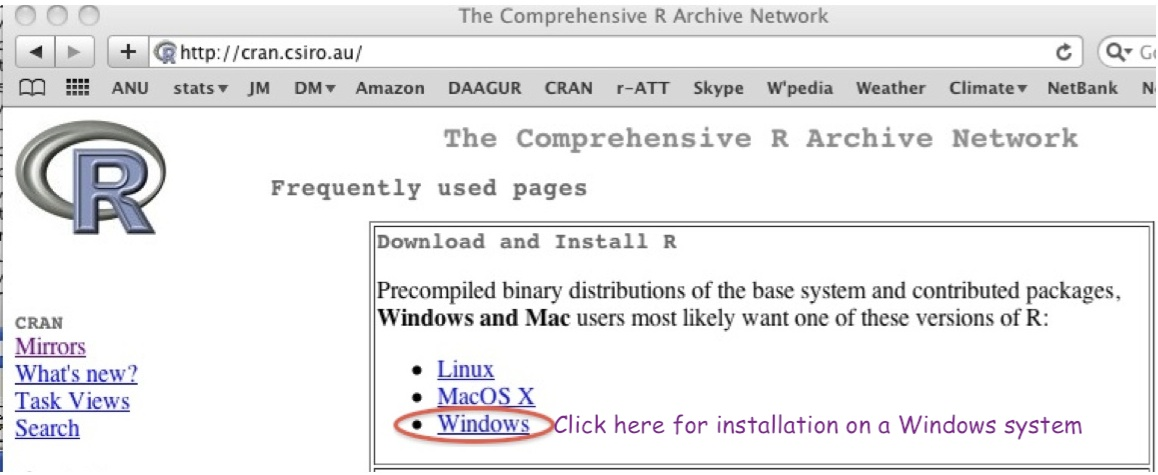
\includegraphics{figs-inc/01i-cran.jpg}
}
\vspace*{2pt}

\fbox{

\includegraphics{figs-inc/01i-base.jpg}
}
\vspace*{2pt}

\fbox{
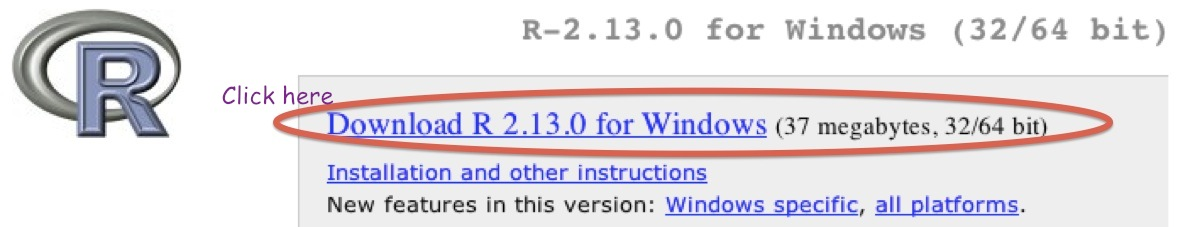
\includegraphics{figs-inc/01i-download.jpg}
}
\caption{This shows a sequence of clicks that will download
  the R installation file from \url{cran.csiro.edu}. At the time of writing,
  the website will offer R-3.4.3 rather than R-2.13.0. The site
  \url{cran.csiro.edu} is one of two Australian CRAN (Comprehensive R Archive
  Network) sites. The other is:
  \url{http://cran.ms.unimelb.edu.au/}}
\end{figure}

\begin{marginfigure}
\begin{center}
\begin{minipage}[c]{0.8\textwidth}

\includegraphics{figs-inc/01i-icons.jpg}
\end{minipage}
\end{center}
\caption{On 64-bit Windows systems the default installation
process creates two icons, one for 32-bit R and one for 64-bit R.
Additional icons can be created as desired.
}
\end{marginfigure}

Click on the downloaded file to start installation.  Most users will
want to accept the defaults.  The effect is to install the R base
system, plus recommended packages, with a standard ``off-the-shelf''
setup.  Windows users will find that one or more desktop R icons have
been created as part of the installation process.

Depending on the intended tasks, it may be necessary to install
further packages. Section \ref{sec:pkgs} describes alternative
ways to install packages.

An optional additional step is to install RStudio.
\marginnote{Clicking on the RStudio icon to start a session will at
  the same time start R. RStudio has its own command line interface,
  where users can type R commands.}  RStudio has abilities that
help in managing workflow, in navigating between projects, and in
accessing R system information.  See Chapter \ref{ch:rstudio}.

\section{First steps}\label{sec:step1}

\marginnote{Readers who have RStudio running can type their commands
in the RStudio command line panel.}
Click on an R icon to start an R session.  This opens an R command
window, prints information about the installed version of R, and
gives a command prompt.

\begin{figure}
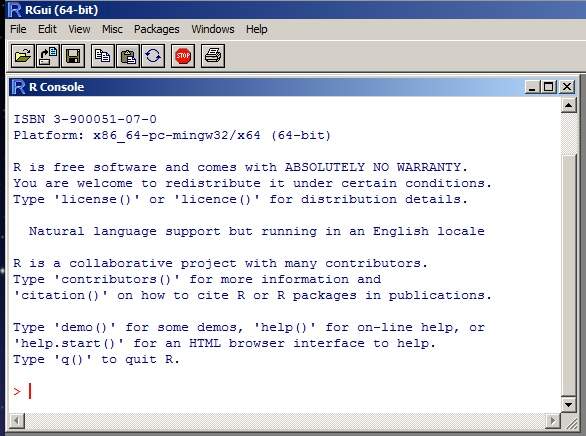
\includegraphics[trim=0 18 0 0]{figs-inc/01i-gui.jpg}
\caption{Windows command window at startup. This shows the default MDI
  (multiple display) interface. For running R from the R Commander,
  the alternative SDI (single display) interface may be required, or
  may be preferable.  The Mac GUI has a SDI type interface; there is
  no other option.}
\end{figure}

\noindent
The \texttt{$>$} prompt that appears on the final line
is an invitation to start typing R commands:

Thus, type \txtt{2+5} and press the Enter key.
The display shows:
\begin{knitrout}
\definecolor{shadecolor}{rgb}{0.969, 0.969, 0.969}\color{fgcolor}\begin{kframe}
\begin{alltt}
\hlstd{> }\hlnum{2}\hlopt{+}\hlnum{5}
\end{alltt}
\begin{verbatim}
[1] 7
\end{verbatim}
\end{kframe}
\end{knitrout}
\noindent
\marginnote[-1.0cm]{The \margtt{[1]} says, a little strangely, ``first
  requested element will follow''. Here, there is just one element.}
The result is 7. The output is immediately followed by the \txtt{>}
prompt, indicating that R is ready for another command.

Try also:
\marginnote[48pt]{Typing \margtt{result} on the
command line has printed the value 7.}
\begin{knitrout}
\definecolor{shadecolor}{rgb}{0.969, 0.969, 0.969}\color{fgcolor}\begin{kframe}
\begin{alltt}
\hlstd{> }\hlstd{result} \hlkwb{<-} \hlnum{2}\hlopt{+}\hlnum{5}
\hlstd{> }\hlstd{result}
\end{alltt}
\begin{verbatim}
[1] 7
\end{verbatim}
\end{kframe}
\end{knitrout}

\marginnote[7pt]{Technically, the \textit{workspace} is one of a
  number of \textit{databases} where objects may be stored.}
The object \margtt{result} is stored in the \textit{workspace}.
The {\em workspace} holds objects that the user has created or input,
or that were there at the start of the session and not later removed

Type \txtt{ls()} to list the objects in the workspace, thus:
\begin{knitrout}
\definecolor{shadecolor}{rgb}{0.969, 0.969, 0.969}\color{fgcolor}\begin{kframe}
\begin{alltt}
\hlstd{> }\hlkwd{ls}\hlstd{()}
\end{alltt}
\begin{verbatim}
[1] "result"
\end{verbatim}
\end{kframe}
\end{knitrout}
\marginnote[-24pt]{The object \margtt{result} was added to
a previously empty workspace.}

Figure \ref{fig:cmds} shows, with annotations, the screen as
it appears following the above sequence of commands.

\begin{figure}
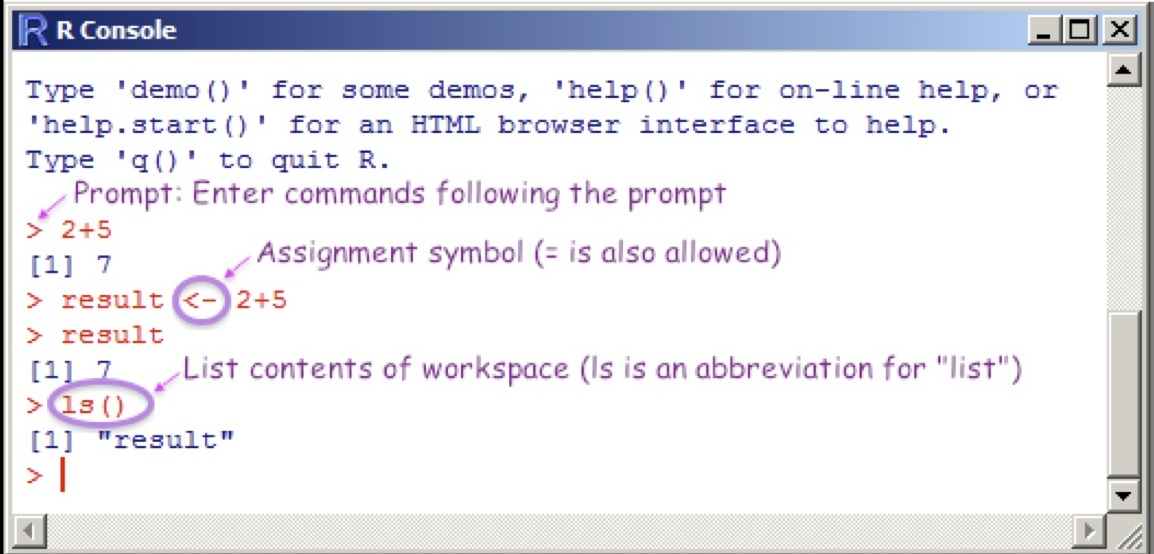
\includegraphics{figs-inc/01i-cmds.jpg}
\caption{This shows the sequence of commands that are demonstrated in
  the text, as they appear on the screen, with added
  annotation.\label{fig:cmds}}
\end{figure}

An R session is structured as a hierarchy of databases. Functions that
were used or referred to above --- such as \txtt{ls()} -- are from a
database or {\em package} that is part of the R system.  Objects that
the user has created or input, or that were there at the start of the
session and not later removed, are stored in the {\em workspace}.

\marginnote[12pt]{Technically, the R system refers to the workspace
as \txtt{.Globalenv}.}
The workspace is the user's database for the duration of a session.
It is a volatile database, i.e., it will disappear if not explicitly
saved prior to or at the end of the session.

\subsection{Points to note}
\noindent
\fbox{\parbox{\textwidth}{\vspace*{-9pt}
\begin{tabbing}
Demonstrations\= \txtt{example(plot)} x\= \kill
Printing \> Typing the name of an object (and pressing \underline{Enter})\\
\> displays (prints) its contents.\\[4pt]
Quitting \> To quit, type \txtt{q()}, (not \txtt{q})\\[4pt]
Case matters \> \txtt{volume} is different from \txtt{Volume}
% Examples \> To run examples from a help page, type, e.g.\\
%  \> \txtt{example(plot)} \> \txtt{\# Example from help(plot)}\\[4pt]
\end{tabbing}
\vspace*{-9pt}
}}
\vspace*{9pt}

Typing the name of an object (and pressing the \underline{Enter} key)
causes the printing of its contents, as above when \txtt{result} was
typed.  This applies to functions also. Thus type \txtt{q()} in order
to quit, not \txtt{q}.\footnote{Typing \txtt{q} lists the code for the
  function.}  One types \txtt{q()} because this causes the function
\txtt{q} to spring into action.

Upon typing \txtt{q()} and pressing the Enter key, a message will ask
whether to save the workspace image.\sidenote{Such an {\em image}
allows reconstruction of the workspace of which it forms an image!}
Clicking Yes (usually the safest
option) will save the objects that remain in the workspace -- any that
were there at the start of the session (unless removed or overwritten)
and any that have been added since.  The workspace that has been thus
saved is automatically reloaded when an R session is restarted in the
working directory to which it was saved.

\begin{figure}
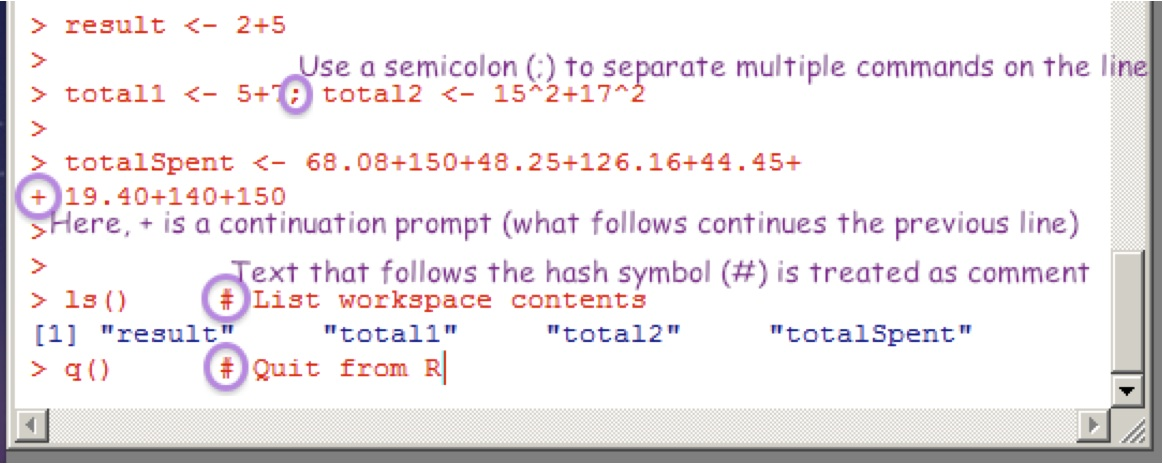
\includegraphics{figs-inc/01i-cmds1.jpg}
\caption{Note the use of the special characters: \txtt{;} to separate
  multiple commands on the one line, \txtt{+} (generated by the
  system) to denote continuation from previous line, and \txtt{\#} to
  introduce comment that extends to end of line.\label{fig:cmds1}}
\end{figure}

Note that for names of R objects or commands, case is significant.
Thus \txtt{Myr} (millions of years, perhaps) differs from \txtt{myr}.
For file names,\sidenote[][-28pt]{Under Windows case
is ignored. For Unix case does distinguish.
(Mac OS X Unix is a partial exception.)} the operating system
conventions apply.

Commands may, as demonstrated in Figure \ref{fig:cmds1}, continue over
more than one line. By default, the continuation prompt is \txtt{+}.
As with the \txtt{>} prompt, this is generated by R, and appears on
the left margin.  Including it when code is entered will give an
error!  \marginnote[-30pt]{Here is a command that extends over two lines:\\
  \margtt{> result <-}\\
  \margtt{+ 2+5} }

\subsection{Some further comments on functions in R}

\marginnote{R is a functional language. Whenever a command is entered,
  this causes a function to run. Addition is implemented as a
  function, as are other such operations.} Common functions that users
  should quickly get to know include \margtt{print()}, \margtt{plot()}
  and \margtt{help()}.  Above, we noted the function \txtt{q()}, used
  to quit from an R session.

Consider the function \txtt{print()}. One can explicitly invoke it to print the
number 2 thus:
\begin{knitrout}
\definecolor{shadecolor}{rgb}{0.969, 0.969, 0.969}\color{fgcolor}\begin{kframe}
\begin{alltt}
\hlkwd{print}\hlstd{(}\hlnum{2}\hlstd{)}
\end{alltt}
\begin{verbatim}
[1] 2
\end{verbatim}
\end{kframe}
\end{knitrout}
Objects on which the function will act are placed inside the round
brackets.  Such quantities are known as {\em arguments} to the function.

An alternative to typing \txtt{print(2)} is to
type \txtt{2} on the command line.  The function \txtt{print()}
is then invoked implicitly:
\begin{knitrout}
\definecolor{shadecolor}{rgb}{0.969, 0.969, 0.969}\color{fgcolor}\begin{kframe}
\begin{alltt}
\hlnum{2}
\end{alltt}
\begin{verbatim}
[1] 2
\end{verbatim}
\end{kframe}
\end{knitrout}

\subsection{Help information}\label{ss:ch1-help}

Included on the information that appeared on the screen when R started
up, and shown in Figures \ref{fig:cmds} and \ref{fig:cmds1}, were brief
details on how to access R's built-in help information:
{\small
\begin{verbatim}
Type 'demo()' for some demos, 'help()' for on-line help, or
'help.start()' for an HTML browser interface to help.
\end{verbatim}
}
\noindent
The shorthand \txtt{?plot} is an alternative to typing
\txtt{help(plot)}.

Replace `\txtt{?}' by `\txtt{??}' for a wider search.  This invokes
the function \txtt{help.search()}, which looks for a partial match
in the title or concept fields as well as in the name.
\begin{marginfigure}[-15pt]
Examples of use of \txtt{??}:\\[-5pt]
\begin{knitrout}
\definecolor{shadecolor}{rgb}{0.969, 0.969, 0.969}\color{fgcolor}\begin{kframe}
\begin{alltt}
\hlopt{??}\hlstd{Arithmetic}
\hlopt{??}\hlstd{base}\hlopt{::}\hlstd{Arith}
  \hlcom{# Search base R only}
\end{alltt}
\end{kframe}
\end{knitrout}
\end{marginfigure}

R has extensive built-in help information.  Be sure to check it out
as necessary.  Section \ref{sec:workinghelp} has further details on
what is available, beyond what you can get by using the help function.

\subsection{The working directory}\label{ss:workdir}

Associated with each session \marginnote{Under Windows, if R is
  started by clicking on an R icon, the working directory is that
  specified in the \underline{Start in} directory specified in the icon
  Preferences.  Subsection \ref{sec:fine-tune} has details on how to
specify the  \underline{Start in} directory for an icon.}
is a working directory where R will by default look
for files.  In particular:
\begin{itemize}
\item If a command inputs data from a file into the
workspace and the path is not specified, this is where R
will look for the file.
\item If a command outputs results to a file, and the path is not specified,
this is where R will place the file.
\item Upon quitting a session, the ``off-the-shelf'' setup will ask
  whether to save an ``image'' of the session. 
\marginnote{When R finds a {\bf .RData} file in the working
  directory at startup, that file will, in an off-the-shelf setup, 
  be used to restore the workspace.}
  Answering
  ``Yes'' has the result that the contents of the workspace are saved
  into a file, in the working directory, that has the name {\bf
    .RData}.  
\end{itemize}

For regular day to day use of R,
it is advisable to have a separate working
directory for each different project.
RStudio users will be asked to specify
a working directory when setting up a new ``project''.

\section{Installation of R Packages}\label{sec:pkgs}
\marginnote[10pt]{ A fresh install of R packages is typically required
  when moving to a new major release (e.g., from a 3.0 series release
  to a 3.1 series release).}

\noindent
\fbox{
  \parbox{\linewidth}{ \noindent
\textbf{Installation of R Packages (Windows \& MacOS X)} \\[3pt]
Start R (e.g., click on the R icon). Then use the relevant menu item to
install packages via an internet connection. This is (usually) easier than
downloading, then installing.\\[6pt]
For command line instructions to install packages, see below.
}}
\vspace*{6pt}

The functions that R provides are organised into packages.  The
packages that need to be installed, additional to those that come with
the initial ready-to-run system, will vary depending on individual
user requirements.  The GUIs --- MacOS X, Windows or Linux --- make
package installation relatively straightforward.

\subsection*{Installation of packages from the command line}

To install the R Commander from the command line, enter:
\marginnote{By default, a CRAN mirror is searched for the required
  package.  Refer back to the introduction for brief comments on
  CRAN.  Subsection \ref{ss:installpack} gives details of
  alternatives to CRAN. Note in particular the Bioconductor
  repository.}
\begin{knitrout}
\definecolor{shadecolor}{rgb}{0.969, 0.969, 0.969}\color{fgcolor}\begin{kframe}
\begin{alltt}
\hlkwd{install.packages}\hlstd{(}\hlstr{"Rcmdr"}\hlstd{,} \hlkwc{dependencies}\hlstd{=}\hlnum{TRUE}\hlstd{)}
\end{alltt}
\end{kframe}
\end{knitrout}
The R Commander has a number of dependencies, i.e., packages that
need to be installed for the R Commander to run.  Graphics packages
that are dependencies include \textit{rgl} (3D dynamic graphics),
\textit{scatterplot3d}, \textit{vcd} (visualization of categorical
data) and \textit{colorspace} (generation of color palettes, etc).

\subsection*{Installation of Bioconductor packages}
\marginnote[10pt]{For installation of Bioconductor packages from the GUI,
  see Subsection \ref{sec:repos}.}  To set your system up for use of
Bioconductor packages, type:
\begin{knitrout}
\definecolor{shadecolor}{rgb}{0.969, 0.969, 0.969}\color{fgcolor}\begin{kframe}
\begin{alltt}
\hlkwd{source}\hlstd{(}\hlstr{"http://bioconductor.org/biocLite.R"}\hlstd{)}
\hlkwd{biocLite}\hlstd{()}
\end{alltt}
\end{kframe}
\end{knitrout}
Additional packages can be installed thus:
\begin{knitrout}
\definecolor{shadecolor}{rgb}{0.969, 0.969, 0.969}\color{fgcolor}\begin{kframe}
\begin{alltt}
\hlkwd{biocLite}\hlstd{(}\hlkwd{c}\hlstd{(}\hlstr{"GenomicFeatures"}\hlstd{,} \hlstr{"AnnotationDbi"}\hlstd{))}
\end{alltt}
\end{kframe}
\end{knitrout}
See further \url{http://www.bioconductor.org/install/}.

\section{Summary}
\begin{itemizz}
\item[] One use of R is as a calculator, to evaluate arithmetic
expressions. Calculations can be carried out in parallel, across all
elements of a vector at once.

\item[] The R Commander GUI can be helpful in getting quickly into use
  of R for many standard purposes.  It may, depending on requirements,
  be limiting for serious use of R.

\item[] Use \txtt{q()} to quit from an R session. To retain objects in
  the workspace, accept the offer to save the workspace.
\end{itemizz}

